\documentclass{beamer}
\usepackage[T1]{fontenc}
\usepackage[utf8]{inputenc}
\usepackage[dvipdfm]{graphicx}
\usepackage{graphics,latexsym}
\usepackage{graphicx}
\usepackage{amsmath}
\usepackage{natbib}
\usepackage[dvips]{color}
\usepackage{subfigure}
\usepackage{verbatim}
\usetheme{Warsaw}
\usecolortheme{default}
\useoutertheme{shadow}
\useinnertheme{rectangles}

\bibpunct{(}{)}{;}{a}{,}{,}

\title[Inference in HBNs]{Inference in Hybrid Bayesian Networks}
\subtitle{state-of-the-art}
\author[Carlos Badenes]{{Carlos Badenes}\\
{\small Computational Intelligence Group, Departamento de Inteligencia Artificial, Universidad Polit\'ecnica de Madrid, Spain}}
\date{}

\begin{document}

\frame{\titlepage}

\begin{frame}
	 \frametitle{Hybrid Bayesian Networks}
	\begin{itemize}
  	  \item Hybrid models are used for representing uncertainty in domains containing not only discrete variables, but also continuous such as distance, temperature or location.
  	\end{itemize}
	\begin{figure}
		  	\centering
    			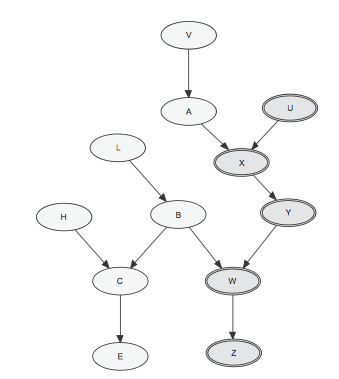
\includegraphics[width=0.4\textwidth]{polytree.png}
  			\caption{Hybrid Bayesian Network}
		\end{figure}
\end{frame}

\begin{frame}
	   \frametitle{Challenges in HBNs}
	\begin{itemize}
	  \item Continuous and discrete variables
	  \item Accuracy
          \item Performance
  	\end{itemize} 
	\begin{figure}
		  	\centering
    			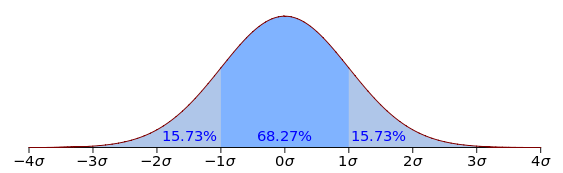
\includegraphics[width=0.3\textwidth]{pdfunction.png}
  			\caption{probability density function}
		\end{figure}
\end{frame}

\begin{frame}
	   \frametitle{Probability in HBNs}
	\begin{itemize}
	  \item Heskes and Zoeter (2003): Generalized Belief propagation to approximate inference in HBNs. $ mean: E[x], covariance: E[(x-E[x])(y-E[y])]$
	 \item Schrempf and Hanebeck, 2004 considered that using  first two moments is a drawback
  	\end{itemize} 
		\begin{figure}
		  	\centering
    			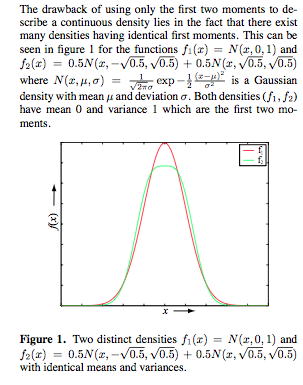
\includegraphics[width=0.4\textwidth]{HBM-2004.png}
  			\caption{Schrempf and Hanebeck, 2004}
		\end{figure}
\end{frame}

\begin{frame}
	   \frametitle{Probability in HBNs }
	   \begin{itemize}
	  	\item Deterministic Variables: Barry R. Cobb and Prakash P. Shenoy, 2004
		\begin{figure}
		  	\centering
    			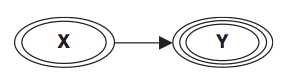
\includegraphics[width=0.2\textwidth]{deterministic.png}
  			\caption{conditionally deterministic variable}
		\end{figure}
	 	\item Continuous variables not normally distributed with \textit{Mixtures of Truncated Exponentials (MTE)} potentials: Barry R. Cobb and Prakash P. Shenoy, 2005
		\begin{figure}
		  	\centering
    			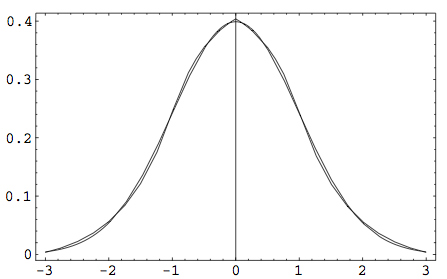
\includegraphics[width=0.2\textwidth]{mte.png}
  			\caption{MTE approximation over on the standard normal distribution}
		\end{figure}
		\item Discrete and continuous variables with \textit{Mixture of Gaussians (MoG)} BNs: Barry R. Cobb and Prakash P. Shenoy, 2006
  	\end{itemize} 	
\end{frame}

\begin{frame}
	\frametitle{HLBP}

	\begin{itemize}
		\item \textit{Hybrid Loopy Belief Propagation(HLBP)}: Changhe Yuan and Marek Druzdzel, 2006
	\end{itemize}
	\begin{figure}
		  	\centering
    			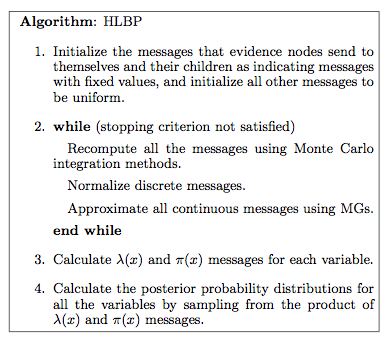
\includegraphics[width=0.4\textwidth]{hlbp.png}
  			\caption{the Hybrid Loopy Belief Propagation algorithm}
	\end{figure}
\end{frame}

\begin{frame}
	\frametitle{DMP}
	\begin{itemize}
		\item \textit{Direct Message Passing for Hybrid Bayesian Network (DMP-HBN)}: Wei Sun and KC Chang, 2010 
	\end{itemize}
	\begin{figure}
		  	\centering
    			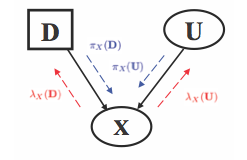
\includegraphics[width=0.4\textwidth]{dmp.png}
  			\caption{continuous node X has discrete parent D and continuous parent U}
	\end{figure}
\end{frame}

\begin{frame}
	\frametitle{Conclusions and future research}
In this short state-of-the-art we have reviewed some of the most important research papers on inference algorithms in Hybrid Bayesian Networks published to date.

The quality of these algorithms, quality as accuracy and performance, is constantly evolving and improving being actually this aspect the main line of research.
\end{frame}

\end{document}